\subsection*{Network Metrics Analysis}
\addcontentsline{toc}{subsection}{Network Metrics Analysis}%
\subsubsection*{Modularity}
As explained in the previous subsection, one data set can be labelled in alternative ways with FSS and FBS binning methods. Consecutively, nonsimilar network motifs will be obtained as output. Those varying textures are a result of the nodes having different degree values within their neighbourhood. 

The degree is a network metric that quantifies one node's links to the other nodes~\cite{Barabasi2016}. It is a way to express the network characteristics. It gives us an idea about the connectivity patterns within the network and allows us to distinguish the group of nodes with a high degree from the nodes with a low degree. 

The nodes clustered together form significant communities or modules in the graph; those patterns give insight into how the data elements are related in the whole network. Modularity is a network measure for community detection and quantifies the strength of community structure in that specific network.

Newman (2006) formulated modularity in his article as
\begin{equation} \tag{1}
	Q = \frac {1} {2 m}\sum_ {ij} (A_{ij} - \frac {k_{i} k_{j}}{2 m}) \
	\frac {s_{i} s_{j} + 1} {2}\ ,
	\label{modularity}
\end{equation}
where the network has an $m$ number of edges, and $A_{ij}$ is the number of edges between vertices $i$ and $j$. $A_{ij}$ is the element of the adjacency matrix introduced in Fig.~\ref{figure-adjacency_graph}. It can be $0$ or $1$. $k_{i}$, and $k_{j}$ are the vertex degrees, and ${k_{i} k_{j}}/{2 m}$ is the expected number of edges between $i$ and $j$ if edges are placed at random. $s_{i}$ and $s_{j}$ are the divided network groups. They are equal to $1$ if $i$ and $j$ belong to the same group and $0$ otherwise. Eq.\eqref{modularity} is used to divide the network into two communities only; however, many networks may contain more than two communities. Therefore, a repeated division into two is adapted: dividing the network into two graphs, then the two sub-graphs further divided into two only if that would maximize $Q$. After first partitioning, the edges falling between the further divided sub-graphs are neglected, leading to the wrong maximization quantity. For this reason, the author introduced the additional contribution $\Delta Q$.~\cite{Newman8577}
% $B_{ij} = A_{ij} - \frac {k_ {i} k_ {j}} {2 m}$\\
% $Q = \frac {1} {4 m} s^{T} Bs = \frac {1} {4 m}\sum_ {i = 
%	1}^{n} (u_ {i}^{T} . s)^{2}\beta_ {i}$\\
% $\Delta Q = \frac {1} {4 m} s^{T} B^{(g)} s$\\
% $B_{ij}^{(g)} = B_{ij} - \delta_{ij}\sum_ {k\in g} B_{ik}$

Since the results obtained with the combination of $Q$ and $\Delta Q$ do not significantly differ from the results obtained only using $Q$, modularity calculations in this work were performed with the latter to lower the computation timing.
\clearpage

\subsubsection*{Different Types of Null Model}
{\color{red} If I have more than two modules, do I conserve the specific number of inter-module edges per module pair? Would a link between module 1 and 2 be shuffled with a link between modules 1 and 3? 
	All the interlinks independent from the number of modules are shuffled in the same set. I did not consider different module interlinks in separate groups. It is a design decision.
	
	In particular, if I do not have the pleasant situation that people usually think of in a modular graph where the connectivity between modules is typically about the same for any pair of modules. But if I have a slightly more realistic situation where module pairs differ very strongly in the way they are interconnected. In real-life data, I often have two challenging modules to separate because they are tightly interconnected and then maybe one or two other modules that are almost not connected to the other modules. That is the part that I do not conserve and might affect the result.
	
	Fixed Degree Sequence random graphs generation, a third one: Conserving Inter-edges and Intra-edges Among Modules random graphs were generated; accordingly, Z-scores were computed among those null models.
	
	I have recomputed my constraint impact analysis pipeline for four production lines with null models: Degrees Fixed and Modularity and different choice of binning in terms of step-size \& bucket-size.
	
	Since plot results vary based on a specific randomization null model, discussing how shuffling was performed is essential. 
	Random graphs were generated, and the below instruments were plotted.
	Modularity vs time windows
	Average modularity for single random graph vs time windows
	Z-scores for modularity randomized null models with modularity conserved vs time windows
	Z-scores for modularity randomized null models with fixed degree sequences vs time windows
	
	
	The cartoon showing how I generated the null models in a pairwise shuffling fashion to prevent ambiguity.}

 \begin{figure}[!ht]
	\begin{center}
		\makebox[\textwidth]{
			\centering
			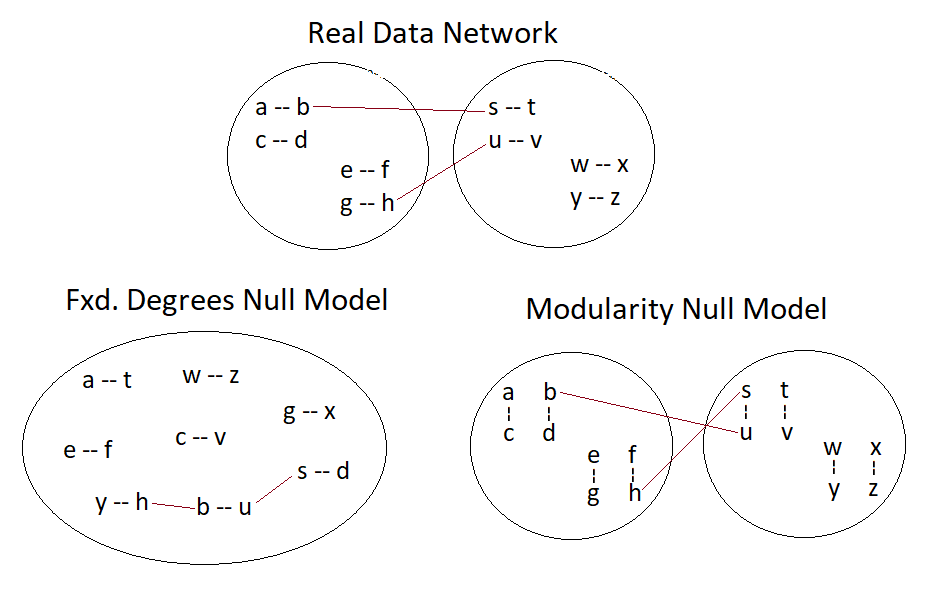
\includegraphics[width=0.6\linewidth]{../images/cartoon-null-model-definitions.png}}
		\caption{Formation of Different Null Models.}
		\label{figure-null_models}
	\end{center}
\end{figure}

{\color{red}
	Introduce hierarchical modularity and its relation with null models.
	
	The full z-score curves are only there because we want to ensure that we don't overlook something. If the full curves are drastically away from zero, then the type of modularity in the real graphs are somewhat different. They are either very asymmetric with respect to the modules or hierarchical or anything else that is very complicated. In some sense, the full curves are just a reference check to whether everything works as expected and whether it is meaningful to discuss modularity. So what we are really looking at is the dashed curves. And I am looking at the z-score only; I am trying to figure out whether the step from FSS to FBS drastically changes the modularity. I am wondering whether we can condense this further to make this information is more accessible.
	
	If the full z-score curves are always close to zero for both different network approaches, would that give us an idea about the modularity? Then it says that the modularity is as we expect the modularity to be. 
	
	If I have a very modular graph and then I randomize it such that I conserve the modularity. Then the comparison of the original modular graph with the randomized modular graphs will lead me to a zero z-score, no matter what the modularity is. 
	
	The dashed line is the more meaningful null model, but we need the other null model because modularity might have strange effects. For example, if the real network has a hierarchical structure, modules within modules within modules, I would still see modularity (positive z-score with respect to the null model behind the full curve) because I am destroying the other type of modularity (nested modularity) in my null model. So in some sense, this is just checking that we have that type of (nested) modularity in deep.
	
	If you have a strongly modular network and each module is in itself modular, then in my null model that preserves modularity, I would destroy that internal modularity of modules. So I would have positive z-scores (full lines would be shifted upwards).
	
	If the full curves are positive, it means we have modules in modules. If the full curves are negative, it means (guessing a bit) that we have big differences in the number of inter-module links. So that some modules are tightly connected while other modules are sparsely connected. And in my null model, this is average. That means that the modularity in the randomized module-conserving networks is actually higher.
	
	Is the dashed curve of FSS higher than the dashed curve of FBS? That's a type of information we should extract from those plots/bar charts.
	
	Performing switch-randomization to a modular graph might fail even due to small details in randomization steps. That failure is probably the reason for the high values of Z-scores in two different plots of Z-scores. If I try to switch-randomize a modular graph, I could imagine a procedure where I take links only from the same module and switch them or links across modules and switch them. And I mixed the sets of intra-module edges and inter-module edges separately. This null model might give a different result in Z-scores.}
\clearpage